\chapter{系统相关技术}
\echapter{Introduction of System Related Technologies}
\section{J2EE的开发框架}
\esection{J2EE development framework}
J2EE技术自从被推出以来就得到了广泛认可和应用,随着多年的技术演变和发展,J2EE技术平台已经日趋成熟,成为当今电子商务的最佳解决方案。相对于微软推出的.NET平台,J2EE继承了Java平台无关性的优点,成为金融,保险,电信等大型应用系统的首选平台方案,如图\ref{2bro}所示。
\begin{figure}[htbp]
  \centering
  % Requires \usepackage{graphicx}
  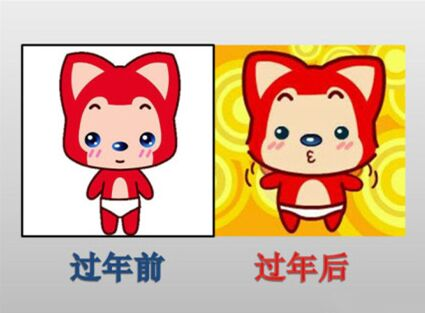
\includegraphics[width=10cm]{3.jpg}\\
  \caption{搞笑图片}\label{2bro}
\end{figure}
\subsection{Struts 2}
\esubsection{Struts 2}
Struts 2最早是Apache Jakarta项目的组成部分,项目创立者希望通过对该项目的研究,改进和提高JSP,Servlet, 标签库以及面向对象的技术水准。 Struts 2采用MVC模式,帮助JAVA开发者利用J2EE开发WEB应用。和其他JAVA架构一样,Struts2也是面向对象的设计,充分发挥了MVC模式 “分离显示逻辑和业务逻辑”的优势。

\renewcommand\arraystretch{1.2}
\begin{table}[htb]
\centering
\caption{My caption}
\label{my-label}
\begin{tabular}{llr}
\hline
\multicolumn{2}{c}{Item} &            \\ \cline{1-2}
Animal     & Description & Price (\$) \\ \hline
Gnat       & per gram    & 13.65      \\
           & each        & 0.01       \\
Gnu        & stuffed     & 92.50      \\
Emu        & stuffed     & 33.33      \\
Armadillo  & frozen      & 8.99       \\ \hline
\end{tabular}
\end{table}

\FloatBarrier
\subsection{Hibernate概述}
\esubsection{Introduction of Hibernate}
Hibernate 是一个开放源代码的对象关系映射框架,对JDBC进行了轻量级的对象封装,使得JAVA程序员可以使用对象编程思维来操作数据库,可以应用在任何使用JDBC的场合,可以在JAVA客户端程序中使用,也可以在Servlet/JSP的Web应用中使用,最厉害的是,它可以在应用EJB的J2EE架构中取代CMP(容器管理持久化),完成数据持久化的重任。


\section{数据库技术}
\esection{Introduction of Database Access Technology}
本文所使用的数据库为开源的MYSQL,MYSQL是一个小型关系数据库管理系统,该数据库的用户已经成千上万了。在本文所实现的CRM系统中需要使用数据库的关键技术就是数据仓库。

数据仓库也是一个数据库,并且大部分都是基于关系型数据库管理系统(RDBMS)设计的,和服务于特定应用软件的交易型数据库不同。数据仓库精简并整合了企业多个数据源的原始数据,其主要用途是为数据访问和企业分析决策之用。数据仓库的整个数据库同交易型数据库是分开的,是各种数据分析工具,信息显示系统的“数据源”,而交易型数据库则是数据仓库的数据源。
\begin{figure}
  \centering%
  \subfigure[第一个小图形]{%
    \label{fig:subfig1}
    
\includegraphics[height=5cm]{4.jpg}}%
  \subfigure[第二个小图形]{%
    \label{fig:subfig2}
    
\includegraphics[height=5cm]{5.jpg}}
  \caption{包含子图形的大图形}
  \label{fig:big1}
\end{figure}

数据仓库虽然同一般交易型数据库采用同样的关系数据库管理系统,但由于建库的目的不同,在设计上是有区别的。在性能上,数据仓库要求快速查询和统计计算,而交易型数据库则要求快速插入或更新,如表\ref{tbl1}所示。
\renewcommand\arraystretch{1.5}
\begin{table}[hbtp]
\centering
\caption{分析型与交易型比较}
\label{tbl1}
\begin{tabular}{|p{3cm}<{\raggedright}|p{5.5cm}<{\raggedright}|}
%\begin{tabular}{|C{3cm}|C{5.5cm}|}
\hline
 & \multicolumn{1}{c|}{\textbf{实体关系特征}} \\ \hline
\textbf{\PreserveBackslash 分析型数据仓库} & 较少连接简单的星型关系链 \\ \hline
\textbf{交易型数据库} & 关系复杂,很多连接 \\ \hline
\end{tabular}
\end{table}


\FloatBarrier
\section{本章小结}
\esection{Summary}
本章主要对本文所实现的银行CRM系统运用的相关关键技术进行了一定的介绍,该系统使用瘦客户端的B/S架构,在J2EE平台上实现。具体的平台使用的是MyEclipse 6.0.所使用的架构是Struts 2+Hibernate+Spring, Struts 2负责MVC模型的建立,Hibernate能让用户用面向对象的思维操作数据库,Spring可以使用JavaBean来完成以前只能由EJB完成的工作。服务器使用的是Apache。
